\documentclass[12pt, titlepage]{article}
%DIF LATEXDIFF DIFFERENCE FILE



\usepackage{booktabs}
\usepackage{tabularx}
\usepackage{hyperref}
\hypersetup{
    colorlinks,
    citecolor=black,
    filecolor=black,
    linkcolor=red,
    urlcolor=blue
}
\usepackage[round]{natbib}
\usepackage{pgfplots}
\usepackage{listings}
\usepackage{xcolor}

\definecolor{codegreen}{rgb}{0,0.6,0}
\definecolor{codegray}{rgb}{0.5,0.5,0.5}
\definecolor{codepurple}{rgb}{0.58,0,0.82}
\definecolor{backcolour}{rgb}{0.95,0.95,0.92}

\newcolumntype{P}[1]{>{\RaggedRight\arraybackslash}p{#1}}

\lstdefinestyle{mystyle}{
    backgroundcolor=\color{backcolour},   
    commentstyle=\color{codegreen},
    keywordstyle=\color{magenta},
    numberstyle=\tiny\color{codegray},
    stringstyle=\color{codepurple},
    basicstyle=\ttfamily\footnotesize,
    breakatwhitespace=false,         
    breaklines=true,                 
    captionpos=b,                    
    keepspaces=true,                 
    numbers=left,                    
    numbersep=5pt,                  
    showspaces=false,                
    showstringspaces=false,
    showtabs=false,                  
    tabsize=2
}
\lstset{style=mystyle}
\pgfplotsset{width=10cm,compat=1.9}

% We will externalize the figures
\usepgfplotslibrary{external}
\tikzexternalize
%% Comments

\usepackage{color}

\newif\ifcomments\commentstrue %displays comments
%\newif\ifcomments\commentsfalse %so that comments do not display

\ifcomments
\newcommand{\authornote}[3]{\textcolor{#1}{[#3 ---#2]}}
\newcommand{\todo}[1]{\textcolor{red}{[TODO: #1]}}
\else
\newcommand{\authornote}[3]{}
\newcommand{\todo}[1]{}
\fi

\newcommand{\wss}[1]{\authornote{blue}{SS}{#1}} 
\newcommand{\plt}[1]{\authornote{magenta}{TPLT}{#1}} %For explanation of the template
\newcommand{\an}[1]{\authornote{cyan}{Author}{#1}}

%% Common Parts

\newcommand{\progname}{SE 4G06} % PUT YOUR PROGRAM NAME HERE
\newcommand{\authname}{Team \#6, Board Gamers
\\ Ilao Michael, ilaom
\\ Bedi Hargun, bedih
\\ Dang Jeffrey, dangj12
\\ Ada Jonah, karaatan
\\ Mai Tianzheng, mait6} % AUTHOR NAMES                  

\usepackage{hyperref}
    \hypersetup{colorlinks=true, linkcolor=blue, citecolor=blue, filecolor=blue,
                urlcolor=blue, unicode=false}
    \urlstyle{same}
                                

%DIF PREAMBLE EXTENSION ADDED BY LATEXDIFF
%DIF UNDERLINE PREAMBLE %DIF PREAMBLE
\RequirePackage[normalem]{ulem} %DIF PREAMBLE
\RequirePackage{color}\definecolor{RED}{rgb}{1,0,0}\definecolor{BLUE}{rgb}{0,0,1} %DIF PREAMBLE
\providecommand{\DIFaddtex}[1]{{\protect\color{blue}\uwave{#1}}} %DIF PREAMBLE
\providecommand{\DIFdeltex}[1]{{\protect\color{red}\sout{#1}}}                      %DIF PREAMBLE
%DIF SAFE PREAMBLE %DIF PREAMBLE
\providecommand{\DIFaddbegin}{} %DIF PREAMBLE
\providecommand{\DIFaddend}{} %DIF PREAMBLE
\providecommand{\DIFdelbegin}{} %DIF PREAMBLE
\providecommand{\DIFdelend}{} %DIF PREAMBLE
\providecommand{\DIFmodbegin}{} %DIF PREAMBLE
\providecommand{\DIFmodend}{} %DIF PREAMBLE
%DIF FLOATSAFE PREAMBLE %DIF PREAMBLE
\providecommand{\DIFaddFL}[1]{\DIFadd{#1}} %DIF PREAMBLE
\providecommand{\DIFdelFL}[1]{\DIFdel{#1}} %DIF PREAMBLE
\providecommand{\DIFaddbeginFL}{} %DIF PREAMBLE
\providecommand{\DIFaddendFL}{} %DIF PREAMBLE
\providecommand{\DIFdelbeginFL}{} %DIF PREAMBLE
\providecommand{\DIFdelendFL}{} %DIF PREAMBLE
%DIF HYPERREF PREAMBLE %DIF PREAMBLE
\providecommand{\DIFadd}[1]{\texorpdfstring{\DIFaddtex{#1}}{#1}} %DIF PREAMBLE
\providecommand{\DIFdel}[1]{\texorpdfstring{\DIFdeltex{#1}}{}} %DIF PREAMBLE
%DIF COLORLISTINGS PREAMBLE %DIF PREAMBLE
\RequirePackage{listings} %DIF PREAMBLE
\RequirePackage{color} %DIF PREAMBLE
\lstdefinelanguage{DIFcode}{ %DIF PREAMBLE
%DIF DIFCODE_UNDERLINE %DIF PREAMBLE
  moredelim=[il][\color{red}\sout]{\%DIF\ <\ }, %DIF PREAMBLE
  moredelim=[il][\color{blue}\uwave]{\%DIF\ >\ } %DIF PREAMBLE
} %DIF PREAMBLE
\lstdefinestyle{DIFverbatimstyle}{ %DIF PREAMBLE
	language=DIFcode, %DIF PREAMBLE
	basicstyle=\ttfamily, %DIF PREAMBLE
	columns=fullflexible, %DIF PREAMBLE
	keepspaces=true %DIF PREAMBLE
} %DIF PREAMBLE
\lstnewenvironment{DIFverbatim}{\lstset{style=DIFverbatimstyle}}{} %DIF PREAMBLE
\lstnewenvironment{DIFverbatim*}{\lstset{style=DIFverbatimstyle,showspaces=true}}{} %DIF PREAMBLE
%DIF END PREAMBLE EXTENSION ADDED BY LATEXDIFF

\begin{document}

\title{Verification and Validation Report \\ An AI-based Approach to Designing Board Games \\ SE 4G06} 
\author{\authname{}}
\date{\today}

\maketitle

\pagenumbering{roman}

\section{Revision History}

\begin{tabularx}{\textwidth}{p{3cm}p{2cm}X}
\toprule {\bf Date} & {\bf Version} & {\bf Notes}\\
\midrule
March 5th & 1.0 & Initial Division of Work\\
March 6th & 1.1 & NFR Eval finished\\
March 7th & 1.2 & Traceability Matricies finished\\
\DIFaddbegin \DIFadd{April 4th }& \DIFadd{1.3 }& \DIFadd{Rev 1 based on feedback \& GitHub issues}\\
\DIFaddend \bottomrule
\end{tabularx}

\DIFdelbegin \DIFdel{~}\DIFdelend \newpage

\DIFaddbegin \tableofcontents


\listoffigures

\newpage

\DIFaddend \section{Symbols, Abbreviations and Acronyms}

\renewcommand{\arraystretch}{1.2}
\begin{tabular}{l l} 
  \toprule		
  \textbf{\DIFdelbegin \DIFdel{symbol}\DIFdelend \DIFaddbegin \DIFadd{Symbol}\DIFaddend } & \textbf{\DIFdelbegin \DIFdel{description}\DIFdelend \DIFaddbegin \DIFadd{Description}\DIFaddend }\\
  \midrule 
  VnV & Verification and Validation \\
  \DIFaddbegin \DIFadd{AI }& \DIFadd{Artificial Intelligence}\\
  \DIFaddend \bottomrule
\end{tabular}\\

\DIFaddbegin \section{\DIFadd{Terminology and  Definitions}}
\DIFadd{This section is expressed in words, not with equations.  It provides the meaning of the different words and phrases used in the domain of the problem.
The terminology is used to introduce concepts from the world outside of the
mathematical model. The terminology provides a real-world connection to give the
mathematical model meaning.
}

\DIFadd{This subsection provides a list of terms that are used in the subsequent
sections and their meaning, with the purpose of reducing ambiguity and making it easier to correctly understand the requirements:
}

\begin{itemize}

\item \textbf{\DIFadd{AI Agent}}\DIFadd{: Refers to the subsystem that has an AI model trained to play the game at hand acting as one of the players of the game.
}

\item \textbf{\DIFadd{Game Engine}}\DIFadd{: Refers to the subsystem that is an abstract representation of the actual game as software.
}

\item \textbf{\DIFadd{Data Visualization}}\DIFadd{: Refers to the subsystem that visualizes Game Engine and AI Agent logs.
}

\item \textbf{\DIFadd{Game State}}\DIFadd{: Refers to the state of the game, which could include player attributes, player score, and game layout. All attributes and characteristics that change throughout a game simulation are stored here.
}

\item \textbf{\DIFadd{Observation Space}}\DIFadd{: Refers to the state of the game that is observable to a Game Agent. (Not all information is available to the Game Agents and can vary from agent to agent)
}

\item \textbf{\DIFadd{Action Space}}\DIFadd{: Refers to the set of moves an AI Agent can take in a particular Game Engine.
}

\item \textbf{\DIFadd{Game Designer}}\DIFadd{: The game designer is the person who is creating the game by coming up with the rules and writing a scenario for the game. The game designer will be the end user of the system to balance the game and improve the design of the game.
}

\end{itemize}

\newpage

\pagenumbering{arabic}

\section{Functional Requirements Evaluation}
\subsection{AI Agents Module}
\subsection{FR Test 1}\DIFaddbegin \label{FRT1} 
\DIFaddend \subsubsection{Test Requirements}
\begin{itemize}
    \item AI Agent responds to the game state 
    \item Display error message
\end{itemize}
\subsubsection{Testing Process}
\begin{enumerate}
    \item Set in \textit{engine.py} a list of size equivalent to the number of players (for the negative case, add an extra player).
    \item Run the simulation in the terminal through \textit{main.py}.
\end{enumerate}
\subsubsection{Expected Results}
\begin{itemize}
    \item Standard output would be the continuous running of the simulation with no error code.
    \item Error message displayed in the terminal indicating invalid observation matrix size.
\end{itemize}
\subsubsection{Actual Results}
\begin{itemize}
    \item \textbf{Positive Test Case:} Simulation ran accordingly and results of the simulation were displayed in the terminal.
    \item \textbf{Negative Test Case:} Invalid matrix size error displayed in the terminal.
\end{itemize}
\subsubsection{Results Analysis}
\item Both test cases passed as expected. 

\subsection{FR Test 2}\DIFaddbegin \label{FRT2} 
\DIFaddend \subsubsection{Test Requirements}
\begin{itemize}
    \item AI Agent is exchangable
    \item Display error message
\end{itemize}
\subsubsection{Testing Process}
\begin{enumerate}
    \item Set each AI agent to an existing policy (set one to a non-existing policy in the negative case) in \textit{ai.py}.
    \item Run the simulation in the terminal through \textit{main.py}.
\end{enumerate}
\subsubsection{Expected Results}
\begin{itemize}
    \item Standard output would be the continuous running of the simulation with no error code.
    \item Error message displayed in the terminal indicating an incorrect policy was chosen.
\end{itemize}
\subsubsection{Actual Results}
\begin{itemize}
    \item \textbf{Positive Test Case:} Simulation ran accordingly and results of the simulation were displayed in the terminal.
    \item \textbf{Negative Test Case:} Invalid policy name error displayed in the terminal.
\end{itemize}
\subsubsection{Results Analysis}
\item Both test cases passed as expected.

\subsection{FR Test 3}\DIFaddbegin \label{FRT3} 
\DIFaddend \subsubsection{Test Requirements}
\begin{itemize}
    \item AI Agent's moves are observable in the environment
\end{itemize}
\subsubsection{Testing Process}
\begin{enumerate}
    \item Run the simulation in the terminal through \textit{main.py}.
\end{enumerate}
\subsubsection{Expected Results}
\begin{itemize}
    \item Standard output is all the AI Agent's moves are logged into a log file in the logs folder.
\end{itemize}
\subsubsection{Actual Results}
\begin{itemize}
    \item \textbf{Positive Test Case:} Simulation ran accordingly and results of the simulation were displayed in the terminal.
\end{itemize}
\subsubsection{Results Analysis}
\item The test case has passed as expected.

\subsection{FR Test 4}\DIFaddbegin \label{FRT4} 
\DIFaddend \subsubsection{Test Requirements}
\begin{itemize}
    \item AI Agent makes valid moves.
    \item The system checks the validity of the move.
\end{itemize}
\subsubsection{Testing Process}
\begin{enumerate}
    \item Run the simulation in the terminal through \textit{main.py}.
\end{enumerate}
\subsubsection{Expected Results}
\begin{itemize}
    \item Standard output is simulation proceeds as normal.
\end{itemize}
\subsubsection{Actual Results}
\begin{itemize}
    \item \textbf{Positive Test Case:} Simulation ran accordingly, results of the simulation were displayed in the terminal and a logs file was produced in the logs folder.
\end{itemize}

\subsection{FR Test 5}\DIFaddbegin \label{FRT5} 
\DIFaddend \subsubsection{Test Requirements}
\begin{itemize}
    \item AI Agent takes observation space as input
\end{itemize}
\subsubsection{Testing Process}
\begin{enumerate}
    \item In \textit{test
    \_engine.py}, initialize an engine and an AI agent, then print both the engine's game state and the observation space of the AI agent.
    \item Run the simulation in the terminal through \textit{test\_engine.py}.
    \item Compare both displayed observation space of the agent and game state of the engine.
\end{enumerate}
\subsubsection{Expected Results}
\begin{itemize}
    \item The observation space of the AI agent is only what the AI agent is expected to see and not the entire game state of the engine. 
\end{itemize}
\subsubsection{Actual Results}
\begin{itemize}
    \item \textbf{Positive Test Case:} Test engine was run successfully and the observation space of the test AI agent was limited to the expected scope.
\end{itemize}
\subsubsection{Results Analysis}
The test case has passed as expected.

\subsection{FR Test 6}\DIFaddbegin \label{FRT6} 
\DIFaddend \subsubsection{Test Requirements}
\begin{itemize}
    \item The simulation is continuous and does not stall on any AI agents' turn
\end{itemize}
\subsubsection{Testing Process}
\begin{enumerate}
    \item Run the simulation with parameters \textit{\texttt{-{}-}
training-num 1 \texttt{-{}-}
test-num 1} in the terminal through \textit{main.py}.
\end{enumerate}
\subsubsection{Expected Results}
\begin{itemize}
    \item Simulation should finish in under 5 minutes.
\end{itemize}
\subsubsection{Actual Results}
\begin{itemize}
    \item \textbf{Positive Test Case:} Simulation was finished in under 1 minute and ran accordingly, results of the simulation were displayed in the terminal and logs file was produced in the logs folder.
\end{itemize}
\subsubsection{Results Analysis}
The test case passed as the simulation finished within the expected time limit.
\subsection{Game Engine Module}

\subsection{FR Test 7} \DIFaddbegin \label{FRT7}
\DIFaddend \subsubsection{Test Requirements}
\begin{itemize}
    \item Game engine is properly initialized
\end{itemize}
\subsubsection{Testing Process}
\begin{enumerate}
    \item Ensure in \textit{engine.py} all starting game entities is initialized in the function \textit{\_\_init\_\_} (for An Aged Contrived, this would include monuments, players, the map and current monuments)
    \item Run the simulation in the terminal through \textit{main.py}.
\end{enumerate}
\subsubsection{Expected Results}
\begin{itemize}
    \item Simulation should complete and generate logs of AI agent actions interacting with the game engine.
\end{itemize}
\subsubsection{Actual Results}
\begin{itemize}
    \item \textbf{Positive Test Case:} Simulation was finished and a log was generated demonstrating proper AI agent actions.
\end{itemize}
\subsubsection{Results Analysis}
The test case has passed.

\subsection{FR Test 8}\DIFaddbegin \label{FRT8} 
\DIFaddend \subsubsection{Test Requirements}
\begin{itemize}
    \item AI Agent makes progress towards an end-game state
\end{itemize}
\subsubsection{Testing Process}
\begin{enumerate}
    \item Initialize a game engine with a game state with an almost completed game in the \textit{test\_engine.py}. 
    \item Assign a very high reward to AI when they complete the reward.
    \item Run the test simulation in the terminal through \textit{test\_engine.py}.
\end{enumerate}
\subsubsection{Expected Results}
\begin{itemize}
    \item Simulation should complete and AI should finish with a very high reward value.
\end{itemize}
\subsubsection{Actual Results}
\begin{itemize}
    \item \textbf{Positive Test Case:} Simulation was finished, the terminal displayed a high reward on the AI agent and the log file displayed the reward.
\end{itemize}
\subsubsection{Results Analysis}
The test case has passed.

\subsection{FR Test 9}\DIFaddbegin \label{FRT9} 
\DIFaddend \subsubsection{Test Requirements}
\begin{itemize}
    \item Game state changes accordingly to AI Agent moves
\end{itemize}
\subsubsection{Testing Process}
\begin{enumerate}
    \item Initialize a game engine with a game state and an AI Agent in the \textit{test\_engine.py}. 
    \item Initialize a game turn on the AI Agent \DIFdelbegin \DIFdel{. }\DIFdelend (energy fill in the case of An Age Contrived)\DIFaddbegin \DIFadd{.
    }\DIFaddend \item Assess the game state of the game engine after the move has been completed. (see if the first monument was filled by the AI agent's action)
\end{enumerate}
\subsubsection{Expected Results}
\begin{itemize}
    \item Game state after AI action is changed accordingly based on the AI action.
\end{itemize}
\subsubsection{Actual Results}
\begin{itemize}
    \item \textbf{Positive Test Case:} Game engine state was properly changed after the AI action (The game engine's monument was filled properly by the AI Agent's energy fill action).
\end{itemize}
\subsubsection{Results Analysis}
The test case has passed.

\subsection{FR Test 10}\DIFaddbegin \label{FRT10} 
\DIFaddend \subsubsection{Test Requirements}
\begin{itemize}
    \item Action list should be consistent throughout the simulation
\end{itemize}
\subsubsection{Testing Process}
\begin{enumerate}
    \item In \textit{env.py}, store and display the available action list for every AI agent in the terminal. 
    \item Check and throw an exception if there are any discrepancies in the action list during the simulation runtime.
\end{enumerate}
\subsubsection{Expected Results}
\begin{itemize}
    \item Simulation should continue running without exception errors and all displayed action lists should be consistent throughout the simulation.
\end{itemize}
\subsubsection{Actual Results}
\begin{itemize}
    \item \textbf{Positive Test Case:} Simulation continued running and all AI Agents' available action lists remained consistent throughout the simulation.
\end{itemize}
\subsubsection{Results Analysis}
The test case has passed.

\subsection{FR Test 11}\DIFaddbegin \label{FRT11} 
\DIFaddend \subsubsection{Test Requirements}
\begin{itemize}
    \item AI Agent and Engine are consistent with each other
\end{itemize}
\subsubsection{Testing Process}
\begin{enumerate}
    \item Initialize a game engine with a game state and an AI agent \textit{test\_engine.py}. (empty monument will have all unfilled tiles)
    \item Initialize a given game move through the AI Agent and display the game state afterwards. (fill monument with Invertible tile)
    \item Run the test simulation in the terminal through \textit{test\_engine.py} repeatedly (at least three times).
    \item Compare each game state after the same AI Agent move was sent to the engine.
\end{enumerate}
\subsubsection{Expected Results}
\begin{itemize}
    \item All game states after the AI Agent move remains consistent.
\end{itemize}
\subsubsection{Actual Results}
\begin{itemize}
    \item \textbf{Positive Test Case:} Each trial's game engine end-game state showed the monument filled with the AI Agent's Invertible tile.
\end{itemize}
\subsubsection{Results Analysis}
The test case has passed.

\subsection{FR Test 12}\DIFaddbegin \label{FRT12} 
\DIFaddend \subsubsection{Test Requirements}
\begin{itemize}
    \item Game engine error handles incorrect data types correctly
\end{itemize}
\subsubsection{Testing Process}
\begin{enumerate}
    \item Initialize a game engine with a game state and an AI agent \textit{test\_engine.py}. 
    \item Initialize a game move with incorrect data types through the AI Agent.
\end{enumerate}
\subsubsection{Expected Results}
\begin{itemize}
    \item Game engine displays to the terminal that a data type provided by the agent is incorrect and the simulation does not continue running.
\end{itemize}
\subsubsection{Actual Results}
\begin{itemize}
    \item \textbf{Negative Test Case:} Data type error was thrown by the engine and simulation was halted.
\end{itemize}
\subsubsection{Results Analysis}
The test case has passed.

\subsection{FR Test 13}\DIFaddbegin \label{FRT13} 
\DIFaddend \subsubsection{Test Requirements}
\begin{itemize}
    \item Game engine error handles illegal moves correctly
\end{itemize}
\subsubsection{Testing Process}
\begin{enumerate}
    \item Initialize a game engine with a game state and an AI agent \textit{test\_engine.py}. 
    \item Initialize an illegal game move through the AI Agent.
\end{enumerate}
\subsubsection{Expected Results}
\begin{itemize}
    \item Game engine displays to the terminal that an illegal move was made by the agent and the simulation does not continue running.
\end{itemize}
\subsubsection{Actual Results}
\begin{itemize}
    \item \textbf{Negative Test Case:} Dead step exception was thrown by the game engine and the simulation did not complete successfully.
\end{itemize}
\subsubsection{Results Analysis}
The test case has passed.

\subsection{Data Visualizer Module}
\subsection{FR Test 14}\DIFaddbegin \label{FRT14} 
\DIFaddend \subsubsection{Test Requirements}
\begin{itemize}
    \item The data visualizer is able to read the JSON log file

\end{itemize}
\subsubsection{Testing Process}
\begin{enumerate}
    \item A simulation log JSON file is created after running the AI simulation.
    \item The data visualizer then is directed to read to the directory/location of the log file.
    \item The data visualizer is executed.
\end{enumerate}
\subsubsection{Expected Results}
\begin{itemize}
    \item The JSON log file is read successfully by the data visualizer and data is displayed on web application.
\end{itemize}
\subsubsection{Actual Results}
\begin{itemize}
    \item \textbf{Positive Test Case:} The data is successfully read by the visualizer and the web application successfully displays the according data in the JSON file.
\end{itemize}
\subsubsection{Results Analysis}
The test case has passed.
\DIFaddbegin 

\DIFaddend \subsection{FR Test 15}\DIFaddbegin \label{FRT15} 
\DIFaddend \subsubsection{Test Requirements}
\begin{itemize}
    \item The data visualizer is able to read the JSON log file
\end{itemize}
\subsubsection{Testing Process}
\begin{enumerate}
    \item Run \textit{npm install} in the \textit{/src/visualization\_v1/} folder.
    \item A simulation log JSON file is created after running the AI simulation.
    \item The data visualizer then is directed by putting the log JSON file into \textit{/src/visualization\_v1/data/} folder and renaming to the file to \textit{game.json}.
    \item The data visualizer is executed with \textit{npm start} and accessed with \textit{http://localhost:3000/}.
\end{enumerate}
\subsubsection{Expected Results}
\begin{itemize}
    \item The JSON log file is read successfully by the data visualizer and data is displayed on the web application.
\end{itemize}
\subsubsection{Actual Results}
\begin{itemize}
    \item \textbf{Positive Test Case:} The data is successfully read by the visualizer and the web application successfully displays the according data in the JSON file.
\end{itemize}
\subsubsection{Results Analysis}
The test case has passed.

\subsection{FR Test 16}\DIFaddbegin \label{FRT16} 
\DIFaddend \subsubsection{Test Requirements}
\begin{itemize}
    \item Data visualizer about to select specific data points
\end{itemize}
\subsubsection{Testing Process}
\begin{enumerate}
    \item Run \textit{npm install} in the \textit{/src/visualization\_v1/} folder.
    \item A simulation log JSON file is created after running the AI simulation.
    \item The data visualizer then is directed by putting the log JSON file into \textit{/src/visualization\_v1/data/} folder and renaming to the file to \textit{game.json}.
    \item The data visualizer is executed with \textit{npm start} and accessed with \textit{http://localhost:3000/}.
    \item On the data visualizer page, try all possible numbers of simulations displayed at once on the page.
\end{enumerate}
\subsubsection{Expected Results}
\begin{itemize}
    \item The JSON log file is read successfully by the data visualizer and data is displayed on the web application. Additionally, the data displayed changes accordingly based on the amount of data points selected by the user.
\end{itemize}
\subsubsection{Actual Results}
\begin{itemize}
    \item \textbf{Positive Test Case:} The data is successfully read by the visualizer and the web application successfully displays the according data in the JSON file. The data populates on the web page according to the number of simulations selected.
\end{itemize}
\subsubsection{Results Analysis}
The test case has passed.
\DIFaddbegin 

\DIFaddend \section{Nonfunctional Requirements Evaluation}

\subsection{Accuracy}
To test accuracy of the system, win rates were compared between AI's using models from that had different levels of training, and checking how their win rates compared (against an AI that only takes random moves) and how long the model was trained for. The expected conclusion was that the longer the model was trained for the higher win rate it would have. The simulation was \DIFdelbegin \DIFdel{ran }\DIFdelend \DIFaddbegin \DIFadd{run }\DIFaddend for a total of 200 times, comparing win rates at intervals of 50 simulations. The higher the AI reward, the more points the AI scored during the game. After running these simulations\DIFaddbegin \DIFadd{, }\DIFaddend the AI's rewards and improved after each interval of training, so we can draw the conclusion that the system became more accurate with more training.
\begin{itemize}
    \item NFR Test 1: \textbf{Pass}
\end{itemize}
\begin{center}
    \begin{tikzpicture}
    \begin{axis}[
        title={NFR Test 1 Results for Accuracy},
        xlabel={Number of Training Simulations},
        ylabel={Average AI Reward per Game},
        xmin=0, xmax=250,
        ymin=0, ymax=300,
        xtick={0,50,100,150,200},
        ytick={0,50,100,150,200,250},
        legend pos=north west,
        ymajorgrids=true,
        grid style=dashed,
    ]
    \addplot[
        color=blue,
        mark=square,
        ]
        coordinates {
        (1,25)(50,100)(100,120)(150,150)(200,170)
        };    
    \end{axis}
    \end{tikzpicture}
\end{center}


\subsection{Usability}
To test the usability of the system, we invited the AI Research Professors and Game Designers to manually test our data visualizers and determine if they can easily navigate and comprehend the data from the charts. We specified all features of our data visualizers and identify how long it takes for the testers to become comfortable with using the tool. The result is that the AI Research Professor and game designers familiarize the manipulation of the data visualizer and remember the workflow of the data visualizer within 20 mins which is significantly less than our expected time for new users to learn how data visualizers. 

\begin{itemize}
    \item NFR Test 2: \textbf{Pass}
\end{itemize}

\subsection{Modularity}
To test the modularity of the system, AI Agents should be able to be swapped with ease and the system should function correctly. AI Agents policies (IE. strategies), are generated as files after a successful execution of the system, the system was \DIFdelbegin \DIFdel{ran }\DIFdelend \DIFaddbegin \DIFadd{run }\DIFaddend twice with different parameters and saved each policy separately. Then the policies were then given as input to the system and was able to function correctly.
\begin{itemize}
    \item NFR Test 2: \textbf{Pass}
\end{itemize}

\subsection{Portability}
To test portability of the system, we tested on different Operating Systems (Mac OS and Windows) and checked if the libraries were able to be installed and if the system could be executed. After clearing all existing libraries and installing a fresh version of Python, the system was able to be installed and executed on both Mac OS and Windows.
\begin{itemize}
    \item NFR Test 4: \textbf{Pass}
    \item NFR Test 5: \textbf{Pass}
    \item NFR Test 6: \textbf{N/A}

\end{itemize}
\subsection{Performance}
To test performance of the system, the system was executed with different number of simulations and timed the length of the runtime. The results were plotted and to ensure the system passes the test, the average runtime per simulation must be less than 5 minutes. The average was well below the targeted of 5 minutes. 

\begin{itemize}
    \item NFR Test 7: \textbf{Pass}
\end{itemize}


\begin{center}
    \begin{tikzpicture}
    \begin{axis}[
        title={NFR Test 7 Results for Performance (Total)},
        xlabel={Number of Total (Training + Testing) Simulations},
        ylabel={Simulation Total Runtime (Minutes)},
        xmin=0, xmax=210,
        ymin=0, ymax=100,
        xtick={0,20,40,60,80,100,120,140,160,180,200},
        ytick={0,10,20,30,40,50,60,70,80,90},
        legend pos=north west,
        ymajorgrids=true,
        grid style=dashed,
    ]
    \addplot[
        color=blue,
        mark=square,
        ]
        coordinates {
        (2,0.33)(10,1.5)(20,4)(80,30)(120,40)(160,55)(200,98)
        };    
    \end{axis}
    \end{tikzpicture}
\end{center}
\begin{center}
    \begin{tikzpicture}
    \begin{axis}[
        title={NFR Test 7 Results for Performance (Average)},
        xlabel={Number of Total (Training + Testing) Simulations},
        ylabel={Average Simulation Runtime (Seconds)},
        xmin=0, xmax=210,
        ymin=0, ymax=30,
        xtick={0,20,40,60,80,100,120,140,160,180,200},
        ytick={0,5,10,15,20,25},
        legend pos=north west,
        ymajorgrids=true,
        grid style=dashed,
    ]
    \addplot[
        color=blue,
        mark=square,
        ]
        coordinates {
        (2,11)(10,9)(20,10)(80,23)(120,20)(160,21)(200,29)
        };    
    \end{axis}
    \end{tikzpicture}
\end{center}


\subsection{Extensibility}
To test extensibility, development time was measured in how long it took to add in new game mechanic. Mechanics varied depending on complexity, but on average it took less than 2 days of development time to develop a new feature, although testing and integration into the entire caused the total time to be over 2 days, causing this test to fail. To further evaluate extensibility of the system, integration and testing time should only be measured since development of mechanics is not a good measurement of the system as a whole, only the game engine.
\begin{itemize}
    \item NFR Test 7: \textbf{Fail}
\end{itemize}
\subsection{Look and Feel}
To test the look and feel of the data visualizer, we invited the game designers and stakeholders to test our data visualizers and conduct a look and feel survey. There are six questions that ask them how they feel about the data visualizer's colors, designs, interactions, and diversity. According to the survey's findings, our users are happy with the data visualizer's user interface and enjoy using it to comprehend data.
\begin{itemize}
    \item NFR Test 9: \textbf{Pass}
\end{itemize}
\newpage
\begin{figure}[!ht]
    \centering
    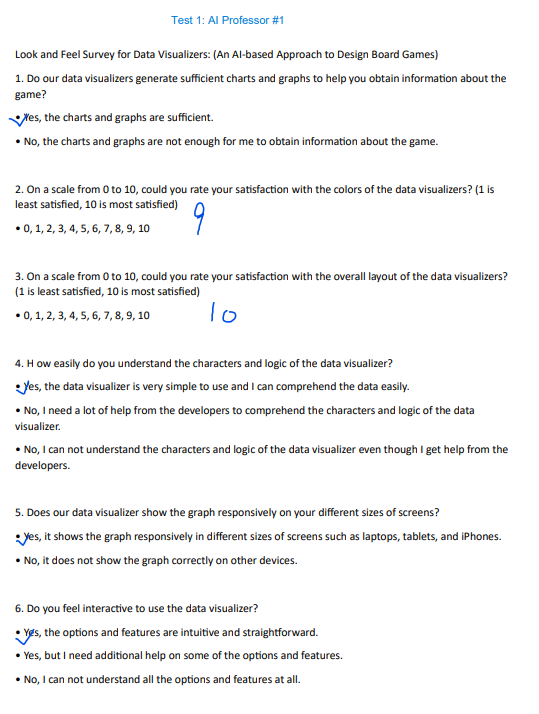
\includegraphics{ai1.png}
    \caption{One of the survey from AI Professor}
    \label{One of the survey from AI Professor}
\end{figure}

\begin{figure}[!ht]
    \centering
    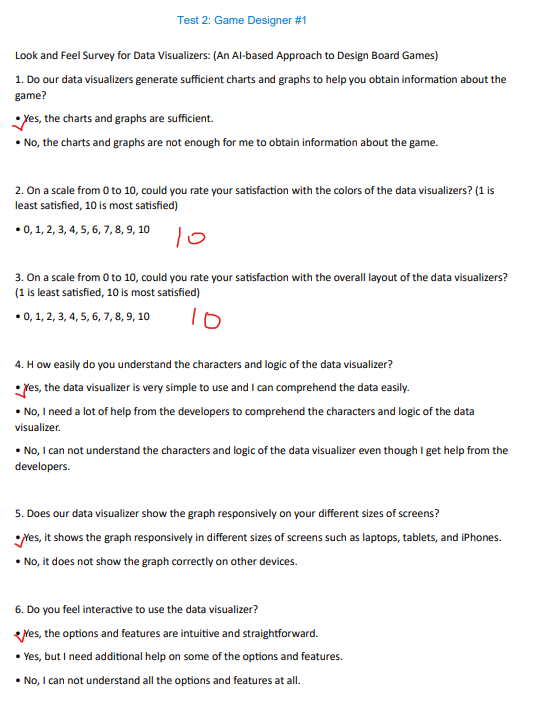
\includegraphics{gd1.png}
    \caption{One of the survey from Game Designer}
    \label{One of the survey from Game Designer}
\end{figure}

\clearpage
\section{Unit Testing}

\subsection{AI & Game Engine Unit Tests}
These functions are under a test class, so self refers to a child of a TestCase class. They use PyTest libraries to run the unit tests and automate them to a degree.
\begin{itemize}
    \item \textbf{Unit Test 1 - FR 7 Test \DIFaddbegin \DIFadd{(\ref{FRT7})}\DIFaddend }: Check whether the game engine initialized correctly. 

 Engine has multiple functions that initializes it and goes back and forth between the AI module and game engine to make sure the AI agents makes choices to initialize the game board. If there is any errors in the initialization, this variable remains False and appropriate exceptions are raised by the game engine.
    \begin{lstlisting}[language=Python]
        def check_engine_initilization(self):
            engine = Engine()
            self.assertTrue(engine.is_initialed)
    
\end{lstlisting}

    \item \textbf{Unit Test 2 - FR 7 Test \DIFaddbegin \DIFadd{(\ref{FRT7})}\DIFaddend }: Check whether the AI agents are initialized correctly in the game engine.

    \begin{lstlisting}[language=Python]
        def check_engine_initilization(self):
            engine = Engine()
            NUM_PLAYERS = 5 #different games can have different players
            self.assertTrue(len(engine.agents) == NUM_PLAYERS)
    
\end{lstlisting}

    \item \textbf{Unit Test 3 - FR1 Test \DIFaddbegin \DIFadd{(\ref{FRT1})}\DIFaddend }: Check whether the AI agents respond to game engine with correct turn type.

    \begin{lstlisting}[language=Python]
        def check_engine_initilization(self):
            engine = Engine()
            current_agent = engine.get_current_agent()
            self.assertTrue(current_agent.turn.turn_type == engine.turn.turn_type)
    
\end{lstlisting}

    \item \textbf{Unit Test 4 - FR2 Test \DIFaddbegin \DIFadd{(\ref{FRT2})}\DIFaddend }: Check whether the new AI agent respond to game engine with correct turn type.

    \begin{lstlisting}[language=Python]
        def check_engine_initilization(self):
            engine = Engine()
            new_agent = Player("agent_name", "default_ai_policy")
            engine.agents[5] = new_agent
            self.assertTrue(engine.agents[5].turn.turn_type == engine.turn.turn_type)
    
\end{lstlisting}

    \item \textbf{Unit Test 5 - FR3 Test \DIFaddbegin \DIFadd{(\ref{FRT3})}\DIFaddend }: Check whether the AI Agent’s moves are observable in the environment. We do this by checking the action\_list in the game engine has action objects inside which are logged to JSON with their English explanations.

    \begin{lstlisting}[language=Python]
        def check_engine_initilization(self):
            engine = Engine()
            current_agent = engine.get_current_agent()
            self.assertTrue(len(engine.get_action_list(current_agent)) > 0)
    
\end{lstlisting}

    \item \textbf{Unit Test 6 - FR5 Test \DIFaddbegin \DIFadd{(\ref{FRT5})}\DIFaddend }: Check whether the AI Agent takes observation space as input. Unit test cannot 100\% test this due to the AI library's input system. However, we can check whether the observation space object is initialized and can check a few key variables to see whether the game engine actually creates a observation space.

    \begin{lstlisting}[language=Python]
        def check_engine_initilization(self):
            engine = Engine()
            observation_space = engine.get_observation_state()
            self.assertTrue(observation_space != None and len(observation_space.map) > 0)
    
\end{lstlisting}

    \item \textbf{Unit Test 7 - FR8 Test \DIFaddbegin \DIFadd{(\ref{FRT8})}\DIFaddend }: Check whether the AI Agent makes progress towards an end-game state. We can check this by looking at the AI agent's reward function and see whether it is greater than 0. Which indicates that the AI actually did moves to earn points to end the game eventually.

    \begin{lstlisting}[language=Python]
        def check_engine_initilization(self):
            engine = Engine()
            current_agent = engine.get_current_agent()
            self.assertTrue(current_agent.reward > 0)
    
\end{lstlisting}

    \item \textbf{Unit Test 8 - FR9 Test \DIFaddbegin \DIFadd{(\ref{FRT9})}\DIFaddend }: Check whether the Game state changes accordingly to AI Agent moves. This is hard to check in unit test level since multiple major sub-systems are involved in changing the game state with the actions. But we can check the AI Agent's observation space is different after the action to infer that there was a change in the game state. 

    \begin{lstlisting}[language=Python]
        def check_engine_initilization(self):
            engine = Engine()
            current_agent = engine.get_current_agent()
            initial_observation_space = current_agent.get_observation_space()
            engine.play_turn() #agent takes action here
            new_observation_space = current_agent.get_observation_space()
            self.assertTrue(initial_observation_space != new_observation_space)
    
\end{lstlisting}    

    \item \textbf{Unit Test 9 - FR10 Test \DIFaddbegin \DIFadd{(\ref{FRT10})}\DIFaddend }: Check whether the  Action list should be consistent throughout the simulation. We can check this by comparing the action list between different turns.

    \begin{lstlisting}[language=Python]
        def check_engine_initilization(self):
            engine = Engine()
            initial_action_list = engine.get_action_list()
            engine.play_turn() #a turn played
            new_action_list = engine.get_action_list()
            self.assertTrue(initial_action_list == new_action_list)
    
\end{lstlisting}  

\end{itemize}
\newpage
\subsection{Data Visualization Unit Tests}
The following tests cover the functions that were created to transform the JSON file received from the game engine module into formats that were needed for the graphs used in this module.
\\\\
Note: JSON Object array refers to an object array with all data from input file, or any modified object array that is return from the the following functions: getAllData, getAllDataExEnd, getDataWithMergedActions. Excluding the first test, all other functions help with \textbf{FR15 Test}, and \textbf{FR16 Test}.

\begin{table}[!ht]
    \label{Data Visualization Unit Testing}
    \centering
    \begin{tabular}{| P{7em} | P{7em} | P{7em} | P{7em} | P{7em} |}
    \hline
        \textbf{Test ID} & \textbf{Function Name} & \textbf{Inputs} & \textbf{Output} & \textbf{Result} \\ \hline
        DV1 - maps to \textbf{FR14 Test \DIFaddbeginFL \DIFaddFL{(\ref{FRT14})}\DIFaddendFL }\te & getAllData & None & JSON object array of the file generated from the Game Engine module & \textcolor{green}{Pass}\\ \hline
        DV2 & getAllData- ExEnd & None & JSON object array with only the data needed for the graphs & \textcolor{green}{Pass} \\ \hline
        DV3 & getDataWith- MergedActions & None & JSON object array that merges the action and action\_details fields into one & \textcolor{green}{Pass} \\ \hline
        DV4 & getSimulation- Data & JSON Object Array, Number of Simulations & Array of Simulations & \textcolor{green}{Pass} \\ \hline
        DV5 & getPlayerData & Object with 1 Simulation data, Player ID  & Object with Simulation data for the specified player & \textcolor{green}{Pass} \\ \hline
        DV6 & getFrequency- Map & None & Object Array with each object having action name and frequency set to 0 & \textcolor{green}{Pass} \\ \hline

        
    \end{tabular}
\end{table}


\begin{table}[!ht]
\begin{tabular}{| P{3em} | P{9em} | P{7em} | P{7em} | P{7em} |}
    \hline
    DV7 & getCountMap & None & Object Array with each object having action name and count set to 0 & \textcolor{green}{Pass} \\ \hline
        DV8 & getFrequencyMapFor- Player & JSON Object Array with merged actions, Number of Simulations, Player ID & Frequency Map Object for the specified player for the specified simulations & \textcolor{green}{Pass} \\ \hline
     DV9 & getCountMapFor- Player & JSON Object Array with merged actions, Number of Simulations, Player ID & Count Map Object for the specified player for the specified simulations & \textcolor{green}{Pass} \\ \hline
        DV10 & getAllNonZeroAct- ions & Frequency/Count Map of a Player & Frequency/Count Map that only has non-zero frequencies/counts & \textcolor{green}{Pass} \\ \hline
        DV11 & getScores & JSON Object Array with merged actions, Number of Simulations & Object with final scores data for the number simulations specified & \textcolor{green}{Pass} \\ \hline
        DV12 & getPlayers & JSON Object Array & Array with sequence of Player IDs & \textcolor{green}{Pass} \\ \hline
\end{tabular}
\end{table}

\newpage
\begin{table}[!ht]
\begin{tabular}{| P{3em} | P{9em} | P{7em} | P{7em} | P{7em} |}
    \hline
        DV13 & getSimulations & JSON Object Array & Array with sequence of simulation IDs & \textcolor{green}{Pass} \\ \hline
        DV14 & getNumberOfMoves & JSON Object Array with merged actions, Number of Simulations, Player ID & Number of moves for the player specified for the number of simulations specified & \textcolor{green}{Pass} \\ \hline
        DV15 & getMap & JSON Object Array with merged actions, Number of Simulations, Player ID & Frequency map for specified player's actions for the number of simulations specified, 2D array of action names where each index is the move number & \textcolor{green}{Pass} \\ \hline
\end{tabular}
\end{table}

\clearpage
\section{Changes Due to Testing}
\DIFaddbegin \DIFadd{Based on the testing, many small bugs and edge cases were discovered in the game engine modules and were fixed. Also, the AI training parameters were improved to meet requirements of runtime and efficiency. Apart from the automated and unit testing, we have also had feedback from our supervisors on data visualizer and training process. Before talking to our supervisors to strategies on AI training, we were using the Apple M1 Pro MacBooks to train the AI agent and we weren't meeting the required training levels. We have tried to improve the training parameters using the manual tests results but weren't able to reach our target goals. Then after discussing it with our supervisors, we got access to Compute Canada supercomputer through their sponsorship and increase the training speed. Then our NFR performance tests started to pass and our system started to show more logical outputs since the AI Agents were smart enough to take logical actions. For data visualizer, we have started with python libraries but after getting supervisor and other user feedback, we have quickly realized that the python did not provide enough graph types to provide meaningful tools to analyze the data generated through our system. So, we have decided to build a web app using React and Apache graphing libraries. At the end, users and supervisor feedback indicated that the visualizer version 1 (React version) was more aligned with our NFRs than visualizer version 0 (python version). Also, based on the feedback, we have made our action space human readable by including English descriptions and tags to them. We have categorized actions which helped with the folder structure in the code and also assigning categories to colour code each action category on the visualizer which improved the usability of our system significantly.
}\DIFaddend \begin{itemize}
    \item \textbf{NFR Test 1}: Changed total simulations to 200, due to length of runtime for 1000 simulations after game engine grew more complex (each simulation took longer to run)
    \item \textbf{NFR Test 6}: Test was not completed as the system was able to be ran on developer's PC's and the computing cluster was not needed.
    \item \textbf{NFR Test 7}: Test was changed to also measure performance against more than 1 simulation and ensuring that the average was less than 1 simulation per 5 minutes
    \item \textbf{FR Test 17}: Related feature was removed after the scope was redefined for the project, thus this test was no longer necessary for the project.
\end{itemize}

\section{Automated Testing}
\subsection{AI Agents & Game Engine Modules}
Since the AI libraries and game engine is written in Python, we have used PyTest libraries to write unit tests. Unit tests described above can run automatically by adding the -test argument (custom made argument in our game engine to handle running all the unit tests) when running the simulation as follow:


\textit{python main.py -test}

\subsection{Data Visualizaton Module}
As this module is developed with JavaScript, we used a popular JavaScript testing framework called Jest for the unit testing. We created mock data as inputs for all the functions and then used their matcher functions like toEqual to validate the results. We also used the code coverage functionality in Jest to measure the code coverage of the tests on the functions. Code Coverage Metrics can be viewed in the \hyperref[Code Coverage Data Visualization]{Code Coverage Metrics section}.

\section{Trace to Requirements}
Full requirement details can be found on the \href{https://github.com/Dorps/aiboardgame/blob/main/docs/SRS/SRS.pdf}{SRS}, under sections 6 and 7. Traceability Matrix below.
\begin{figure}[!h]
    \centering
    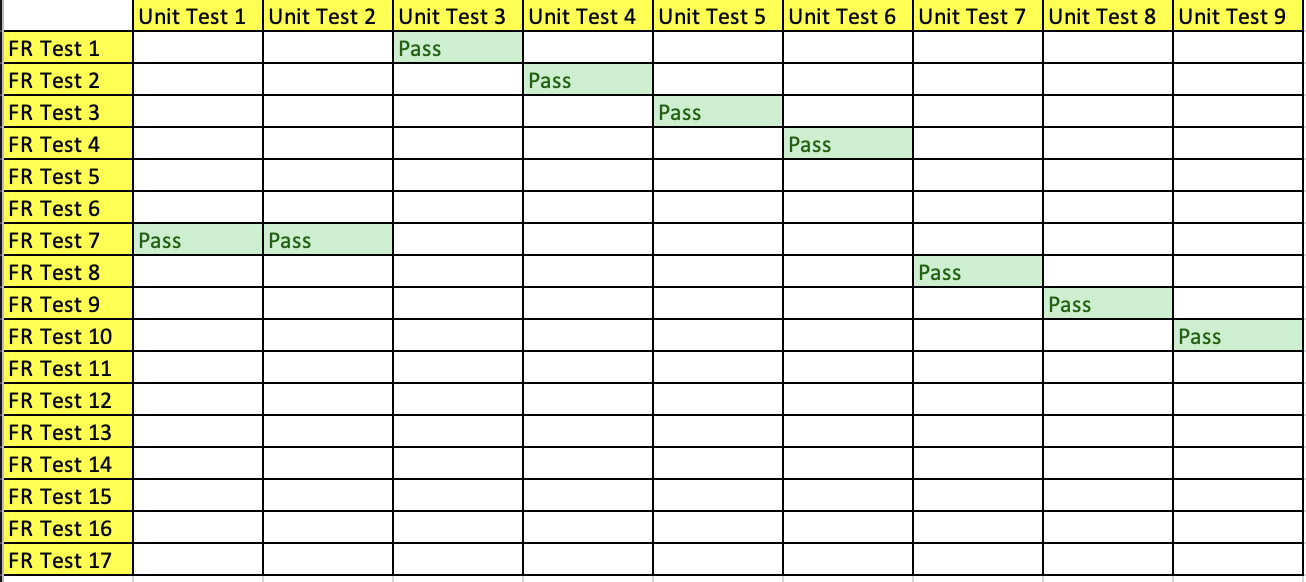
\includegraphics[width=\textwidth]{Unit.png}
    \caption{Unit Tests to Functional Requirement Tests Matrix}
    \label{Functional Requirements to Tests Matrix}
\end{figure}
\begin{figure}[!h]
    \centering
    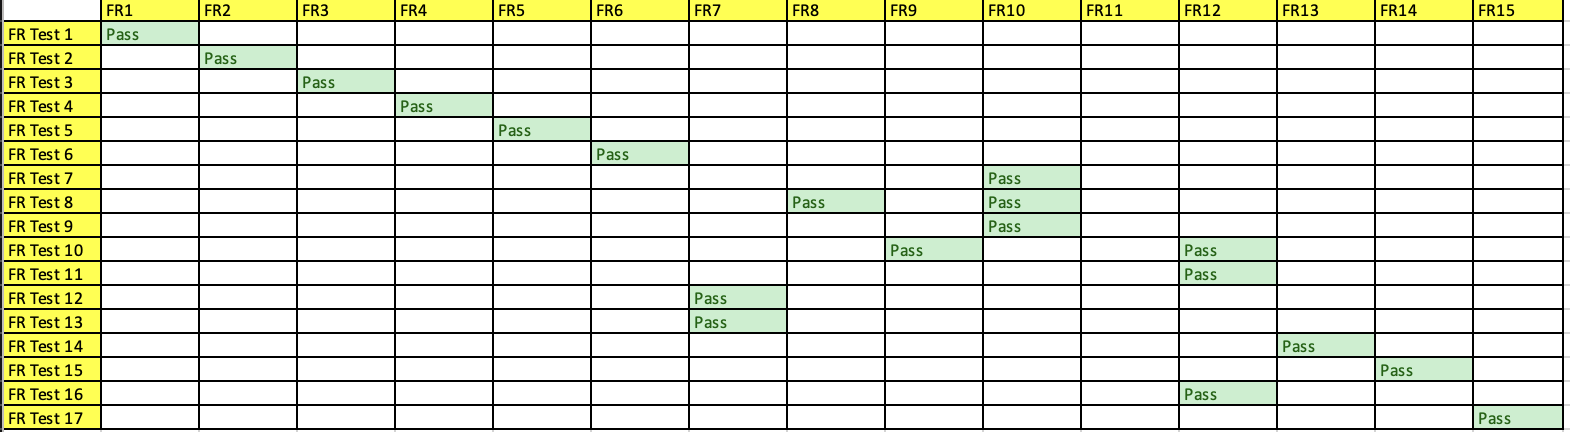
\includegraphics[width=\textwidth]{FR.png}
    \caption{Functional Requirements to Tests Matrix}
    \label{Functional Requirements to Tests Matrix}
\end{figure}
\begin{figure}[!ht]
    \centering
    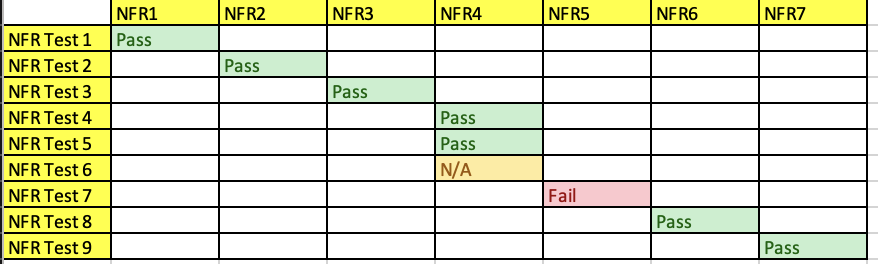
\includegraphics[width=\textwidth]{NFR.png}
    \caption{Non-Functional Requirements to Tests Matrix}
    \label{Non-Functional Requirements to Tests Matrix}
\end{figure}

\clearpage
\section{Trace to Modules}		
Full module details can be found on the \href{https://github.com/Dorps/aiboardgame/blob/main/docs/Design/Design.pdf}{Design Document}. 
\begin{figure}[!ht]
    \centering
    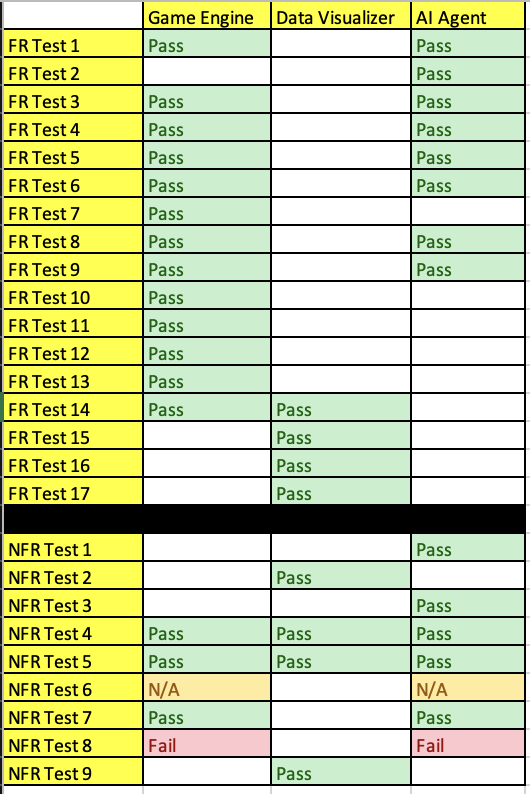
\includegraphics{MG.png}
    \caption{Modules to Tests Matrix}
    \label{Modules to Tests Matrix}
\end{figure}
\section{Code Coverage Metrics}
\subsection{AI Agents & Game Engine Modules}
The unit test coverage is not taken into account since unit tests can only check a very small subset of the game engine due to complex code execution sequence that AI libraries require. So, any code coverage figure would be really low and not really reflect our confidence in the game. Most of our testing is done through looking at the visualization and log files to confirm that the AI outputs are within the game rules and makes sense.
\subsection{Data Visualization Module}
\begin{figure}[!ht]
    \centering
    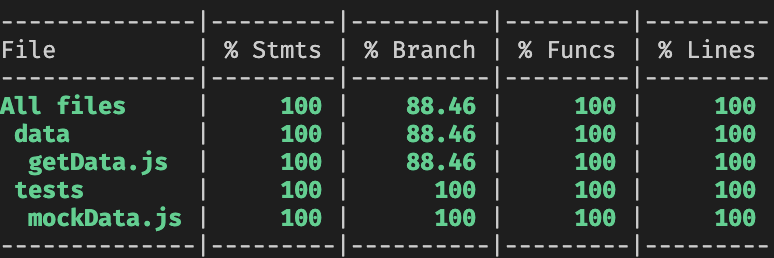
\includegraphics[width=\textwidth]{DataVisualizationCoverage.png}
    \caption{Data Visualization Code Coverage Metrics}
    \label{Data Visualization Code Coverage Metrics}
\end{figure}
\label{Code Coverage Data Visualization}
With our unit testing, we were able to get 100\% statement and function coverage. We achieved 88.46\% branch coverage as we were not able to reach a branch in a sorting function which was used to sort some of the objects and arrays. However, as a group we had decided that we were satisfied with achieving $> 80\%$ coverage on statements, branches and functions. 

\newpage
\section{Reflection}
As a team, we noticed the changes in our verification and validation plan (VnV) and the report had changed in major and minor ways as there was a major difference between writing the plan and report, which would be the finishing of the implementation of our project. Before, planning the verification and validation of our system was very abstract as we were not entirely sure how we would end up implementing the whole system. Currently, we finished the implementation and are able to test directly and have solid test cases to demonstrate the feasible system. The concreteness of the project demonstrates how we have to critically think about what portion of the system we either missed completely in our code coverage or spent too many test cases when it is an obvious piece of code that will self-facilitate itself after implementation on our VnV plan. Furthermore, the focus of the project is the structure of an AI simulation of ANY board game, so many of our test cases are generalized for all board games applied to the system and any unit tests directly related to the game we specifically worked with (An Age Contrived) are omitted from this document. Any specific examples of An Age Contrived for testing are described in brackets in the documents. Another change between the VnV Plan and the VnV Report is the metrics used for testing the Non-Functional Requirements, initially we did not know the performance of our system, so we had a low threshold for how well we wanted it to perform. After building the system, our system performed way higher than expected due to not knowing how the system will run with the given resources. 

    For next time, when writing our VnV plan we will consider of the possible implementation of the system, rather than abstracting some of the tests. This would result in fewer changes for us during the VnV report portion and lead to greater consistency in the report.

\bibliographystyle{plainnat}

\bibliography{../../refs/References}

\end{document}